\documentclass[journal,12pt,twocolumn]{IEEEtran}
\usepackage{setspace}
%\usepackage{gensymb}
\singlespacing
\usepackage[cmex10]{amsmath}
\usepackage{amsthm}
\usepackage{mathrsfs}
\usepackage{txfonts}
%\usepackage{stfloats}
\usepackage{bm}
\usepackage{cite}
%\usepackage{cases}
\usepackage{subfig}
\usepackage{longtable}
%\usepackage{multirow}
%\usepackage{enumitem}
\usepackage{mathtools}
%\usepackage{steinmetz}
%\usepackage{tikz}
%\usepackage{circuitikz}
\usepackage{verbatim}
%\usepackage{tfrupee}
\usepackage[breaklinks=true]{hyperref}
\usepackage{graphicx}
%\usepackage{tkz-euclide}
%\usetikzlibrary{calc,math}
\usepackage{listings}
\usepackage{color}                                            %%
\usepackage{array}                                            %%
\usepackage{longtable}                                        %%
\usepackage{calc}                                             %%
%\usepackage{multirow}                                         %%
\usepackage{hhline}                                           %%
\usepackage{ifthen}                                           %%
\usepackage{lscape}     
\usepackage{multicol}
%\usepackage{chngcntr}
\DeclareMathOperator*{\Res}{Res}
\renewcommand\thesection{\arabic{section}}
\renewcommand\thesubsection{\thesection.\arabic{subsection}}
\renewcommand\thesubsubsection{\thesubsection.\arabic{subsubsection}}
\renewcommand\thesectiondis{\arabic{section}}
\renewcommand\thesubsectiondis{\thesectiondis.\arabic{subsection}}
\renewcommand\thesubsubsectiondis{\thesubsectiondis.\arabic{subsubsection}}
\hyphenation{op-tical net-works semi-conduc-tor}
\def\inputGnumericTable{}                                 %%

\lstset{
%language=C,
frame=single, 
breaklines=true,
columns=fullflexible
}
\begin{document}
\newtheorem{theorem}{Theorem}[section]
\newtheorem{problem}{Problem}
\newtheorem{proposition}{Proposition}[section]
\newtheorem{lemma}{Lemma}[section]
\newtheorem{corollary}[theorem]{Corollary}
\newtheorem{example}{Example}[section]
\newtheorem{definition}[problem]{Definition}
\newcommand{\BEQA}{\begin{eqnarray}}
\newcommand{\EEQA}{\end{eqnarray}}
\newcommand{\define}{\stackrel{\triangle}{=}}
\bibliographystyle{IEEEtran}
\raggedbottom
\setlength{\parindent}{0pt}
\providecommand{\mbf}{\mathbf}
\providecommand{\pr}[1]{\ensuremath{\Pr\left(#1\right)}}
\providecommand{\qfunc}[1]{\ensuremath{Q\left(#1\right)}}
\providecommand{\sbrak}[1]{\ensuremath{{}\left[#1\right]}}
\providecommand{\lsbrak}[1]{\ensuremath{{}\left[#1\right.}}
\providecommand{\rsbrak}[1]{\ensuremath{{}\left.#1\right]}}
\providecommand{\brak}[1]{\ensuremath{\left(#1\right)}}
\providecommand{\lbrak}[1]{\ensuremath{\left(#1\right.}}
\providecommand{\rbrak}[1]{\ensuremath{\left.#1\right)}}
\providecommand{\cbrak}[1]{\ensuremath{\left\{#1\right\}}}
\providecommand{\lcbrak}[1]{\ensuremath{\left\{#1\right.}}
\providecommand{\rcbrak}[1]{\ensuremath{\left.#1\right\}}}
\theoremstyle{remark}
\newtheorem{rem}{Remark}
\newcommand{\sgn}{\mathop{\mathrm{sgn}}}
\providecommand{\abs}[1]{\left\vert#1\right\vert}
\providecommand{\res}[1]{\Res\displaylimits_{#1}} 
\providecommand{\norm}[1]{$\left\lVert#1\right\rVert$}
%\providecommand{\norm}[1]{\lVert#1\rVert}
\providecommand{\mtx}[1]{\mathbf{#1}}
\providecommand{\mean}[1]{E$\left[ #1 \right]$}
\providecommand{\fourier}{\overset{\mathcal{F}}{ \rightleftharpoons}}
%\providecommand{\hilbert}{\overset{\mathcal{H}}{ \rightleftharpoons}}
\providecommand{\system}{\overset{\mathcal{H}}{ \longleftrightarrow}}
%\newcommand{\solution}[2]{\textbf{Solution:}{#1}}
\newcommand{\solution}{\noindent \textbf{Solution: }}
\newcommand{\cosec}{\,\text{cosec}\,}
\providecommand{\dec}[2]{\ensuremath{\overset{#1}{\underset{#2}{\gtrless}}}}
\newcommand{\myvec}[1]{\ensuremath{\begin{pmatrix}#1\end{pmatrix}}}
\newcommand{\mydet}[1]{\ensuremath{\begin{vmatrix}#1\end{vmatrix}}}
\numberwithin{equation}{subsection}
\makeatletter
\@addtoreset{figure}{problem}
\makeatother
\let\StandardTheFigure\thefigure
\let\vec\mathbf
\renewcommand{\thefigure}{\theproblem}
\def\putbox#1#2#3{\makebox[0in][l]{\makebox[#1][l]{}\raisebox{\baselineskip}[0in][0in]{\raisebox{#2}[0in][0in]{#3}}}}
\def\rightbox#1{\makebox[0in][r]{#1}}
\def\centbox#1{\makebox[0in]{#1}}
\def\topbox#1{\raisebox{-\baselineskip}[0in][0in]{#1}}
\def\midbox#1{\raisebox{-0.5\baselineskip}[0in][0in]{#1}}
\vspace{3cm}
\title{EE3025-Assignment 1}
\author{BHUKYA SIDDHU - EE18BTECH11004}
\maketitle
\newpage
\bigskip
\renewcommand{\thefigure}{\theenumi}
\renewcommand{\thetable}{\theenumi}
Download all python codes from 
\begin{lstlisting}
https://github.com/Siddhu27/ee3025_ass1/tree/main/codes
\end{lstlisting}
%
and latex-tikz codes from 
%
\begin{lstlisting}
https://github.com/Siddhu27/ee3025_ass1
\end{lstlisting}
(5.3) The system with h(n) is defined to be stable if 
\begin{align}
\sum_{n=-\infty}^{\infty} \abs{h(n)} < \infty
\end{align} 
Is the system defined by (3.2) stable for impulse response in (5.1)?
\section{Solution}
\textbf{Method I :}
\\
BIBO Stability Criteria : A system is said to be stable, if the bounded input produces the bounded output.\\
Let x(n) be a bounded sequence.So, 
\begin{align}
\abs{x(n)}<M_x
\end{align}
Where $M_x$ is a finite value.From the convolution property,
\begin{align}
 y(n)= \sum_{-\infty}^{\infty}h(k)x(n-k)\\
 \abs{y(n)}= \abs{\sum_{-\infty}^{\infty}h(k)x(n-k)}\\
 \abs{y(n)} \leq M_x\sum_{-\infty}^{\infty}\abs{h(k)} 
\end{align}
Because all x(k) less than $M_x$.\\
As $M_x$ is finite, for $\abs{y(n)}$ to be finite
\begin{align}
\sum_{-\infty}^{\infty}\abs{h(n)} < 
\infty \\
\text{then} \abs{y(n)} \leq M_y < \infty 
\end{align}
Therefore we can say that the output is bounded if the impulse response is absolutely summable.\\
\\
Given difference equation: 
\begin{align}
y(n)+\frac{1}{2}y(n-1) = x(n)+x(n-2) \\
y(n)=0 \text{ for }y<0
\end{align}\\
and the given bounded input is \\
\begin{align}
x(n) = \cbrak{1,1,2,4,3,1}
\end{align} \\
\begin{figure}[h!]
    \centering
    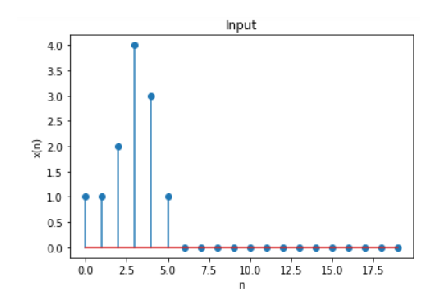
\includegraphics[width=8cm]{./figures/INPUT.eps}
    \caption{Given input}
    \label{xn}
\end{figure}\\
and the output we get,\\
\begin{figure}[h!]
    \centering
    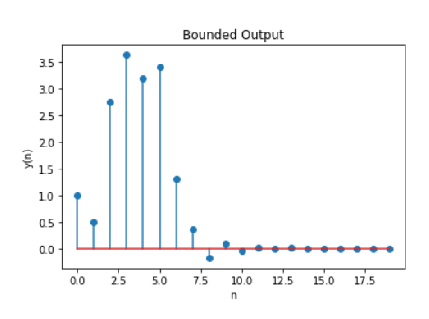
\includegraphics[width=7cm]{./figures/OUTPUT.eps}
    \caption{Bounded output}
    \label{yn}
\end{figure} \\
So we can see that we are getting bounded output for the bounded input.Therefore,
the given system is stable.\\
\textbf{Method 2 :}
\\
Given difference equation,
\begin{align}
y(n)+\frac{1}{2}y(n-1) = x(n)+x(n-2) 
\end{align}\\
By applying Z-transform we get, \\
\begin{align}
Y(z) + \frac{1}{2}z^{-1}Y(z)=X(z) + z^{-2}X(z)\\
Y(z)=\frac{2(z^2+1)}{z(2z+1)}X(z)
\end{align}\\
Therefore H(z) is \\
\begin{align}
H(z) = \frac{2(z^2+1)}{z(2z+1)} \\
H(z) = \frac{1+z^{-2}}{1+\frac{1}{2}z^{-1}}
\end{align}
\begin{align}
H(z)= z^{-1}\sbrak{\frac{1}{1+\frac{1}{2}z^{-1}} + \frac{z^{-2}}{1+\frac{1}{2}z^{-1}}}
\end{align}\\
By applying inverse z-transform we get,\\
\begin{align}
    h(n)=\sbrak{\frac{-1}{2}}^nu(n) + \sbrak{\frac{-1}{2}}^{n-2}u(n-2)
\end{align}\\
As the condition for the system to be stable is
\begin{align}
\sum_{n=-\infty}^{\infty} \abs{h(n)} < \infty
\end{align}\\
By substituting h(n) we get,\\
\begin{align}
\sum_{n=-\infty}^{\infty} \abs{h(n)} &= \sum_{n=-\infty}^{\infty}\abs{\sbrak{\frac{-1}{2}}^nu(n) + \sbrak{\frac{-1}{2}}^{n-2}u(n-2)}
\end{align}
\begin{align}
&= 
\sum_{n=-\infty}^{\infty}\abs{(-1)^n \left( \sbrak{\frac{-1}{2}}^nu(n) + \sbrak{\frac{-1}{2}}^{n-2}u(n-2) \right)}  \\
&= 
\sum_{n=-\infty}^{\infty}\abs{\sbrak{\frac{1}{2}}^nu(n) + \sbrak{\frac{1}{2}}^{n-2}u(n-2)} \\
&=
\sum_{n=-\infty}^{\infty}\sbrak{\frac{1}{2}}^nu(n)+\sum_{n=-\infty}^{\infty}\sbrak{\frac{1}{2}}^{n-2}u(n-2)\\
&=
\sum_{n=0}^{\infty}\sbrak{\frac{1}{2}}^n+\sum_{n=2}^{\infty}\sbrak{\frac{1}{2}}^{n-2}\\
&=
\sbrak{\frac{1}{1-\frac{1}{2}}}+\sbrak{\frac{1}{1-\frac{1}{2}}}\\
&=
2+2\\
&=
4 < \infty
\end{align}\\
As the given system satisfies the stability condition.Therefore, the system is stable.\\
\\
\textbf{Method 3 :}
\\
The condition for the system to be stable is,
\begin{align}
    \sum_{n=-\infty}^{\infty}\abs{h(n)}<\infty
\end{align}
The above equation can be written as,
\begin{align}
    \sum_{n=-\infty}^{\infty}\abs{h(n)}\abs{z^{-n}}_{\abs{z}=1}<\infty\\
    \sum_{n=-\infty}^{\infty}\abs{h(n)z^{-n}}_{\abs{z}=1}<\infty
\end{align}
From triangle inequality,
\begin{align}
   \sum_{n=-\infty}^{\infty}\abs{h(n)z^{-n}}_{\abs{z}=1}<\abs{\sum_{n=-\infty}^{\infty}h(n)z^{-n}}_{\abs{z}=1}
\end{align}
\begin{align}
     \therefore \abs{H(z)}_{\abs{z}=1}<\infty
\end{align}
For the system to be stable unit circle should lie in the ROC of the system.\\
From the equation 1.0.15,
\begin{align}
H(z) &= z^{-1}\sbrak{\frac{1}{1+\frac{1}{2}z^{-1}} + \frac{z^{-2}}{1+\frac{1}{2}z^{-1}}}\\
&=
z^{-1}\sbrak{1-\frac{1}{2z}+\left( \frac{1}{2z} \right)^{2} +.... +z^{-2}\sbrak{1-\frac{1}{2z}+\left( \frac{1}{2z} \right)^{2} +....}}
\end{align}\\
The above expansion is infinite G.P, so the summation is finite if $z\neq0$ and\\
\begin{align}
\abs{\frac{1}{2z}}<1 \implies \abs{z}>\frac{1}{2}
\end{align}\\
From the equation 1.0.33 ROC of the system consists the unit circle.Thus, the given system is stable.\\
\\
Verification through z-plane,\\
\begin{figure}[h!]
    \centering
    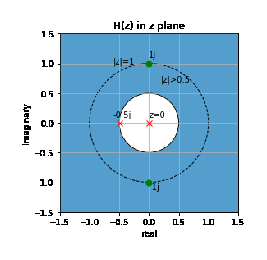
\includegraphics[width=8cm]{./figures/ROC.eps}
    \caption{Plot of H(z) in Z-Plane}
    \label{yn}
\end{figure} \\
From the above plot we can verify that unit circle is lying in the ROC of the system.
Therefore, the system is stable. 







\end{document}

